
\chapter{Differentials}



%87. 
\section{Introduction}

Thus far we have represented the derivative of $y = f(x)$ by the notation

\[
    \frac{dy}{dx} = f'(x).
\]
We have taken special pains to impress on the student that the symbol

\[
    \frac{dy}{dx}
\]
was to be considered not as an ordinary fraction with $dy$ 
as numerator and $dx$ as denominator, but as a single symbol 
denoting the limit of the quotient

\[
    \frac{\Delta y}{\Delta x}
\]
as $\Delta x$ approaches the limit zero.

Problems do occur, however, where it is very convenient to 
be able to give a meaning to $dx$ and $dy$ separately, and it 
is especially useful in applications of the Integral Calculus. 
How this may be done is explained in what follows.

%88. 
\section{Definitions}
%% This section and the next seem very unsatisfactory... 
%% Some is very similar to Hardy's section on Differentials
%% in his ``A course of pure mathematics''
\label{sec:88}

If $f'(x)$ is the derivative of $f(x)$ for a particular value 
of $x$, and $\Delta x$ is an arbitrarily chosen\footnote{The term
``arbitrarily chosen'' essentially means that
the variable $\Delta x$ is independent from the variable
$x$.} %% new
increment of $x$, then the {\it differential} of $f(x)$, denoted 
by the symbol $df(x)$, is defined by the equation
\index{differential}

\begin{equation}
%(A) 
df(x) = f'(x)\Delta x.
\label{eqn:A-88}
\end{equation}
If now $f(x) = x$, then $f'(x) = 1$, and (\ref{eqn:A-88}) reduces to
$   dx = \Delta x$,
showing that when $x$ is the independent variable, 
the differential of $x$ ($= dx$) is identical 
with $\Delta x$. Hence, if $y = f(x)$, (\ref{eqn:A-88}) may in 
general be written in the form

\begin{equation}
%(B) 
dy = f'(x)\, dx.
\label{eqn:B-88}
\end{equation}
The differential of a function equals its derivative multiplied 
by the differential of the independent variable.

On account of the position 
which the derivative $f'(x)$ here occupies, it is sometimes called 
the {\it differential coefficient}. The student should observe the 
important fact that, since $dx$ may be given any arbitrary value 
whatever, $dx$ is independent of $x$. Hence, $dy$ is a function 
of two independent variables $x$ and $dx$.
%% this was a footnote in the text. I have placed it in the
%% text for clarity.

Let us illustrate what this means geometrically.

\begin{figure}[h!]
%\begin{tabular}{cc}
\begin{minipage}{\textwidth}
\begin{center}
%\vspace{1.0 cm}
%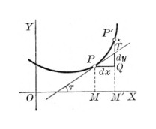
\includegraphics[height=4cm,width=4cm]{differential.eps}
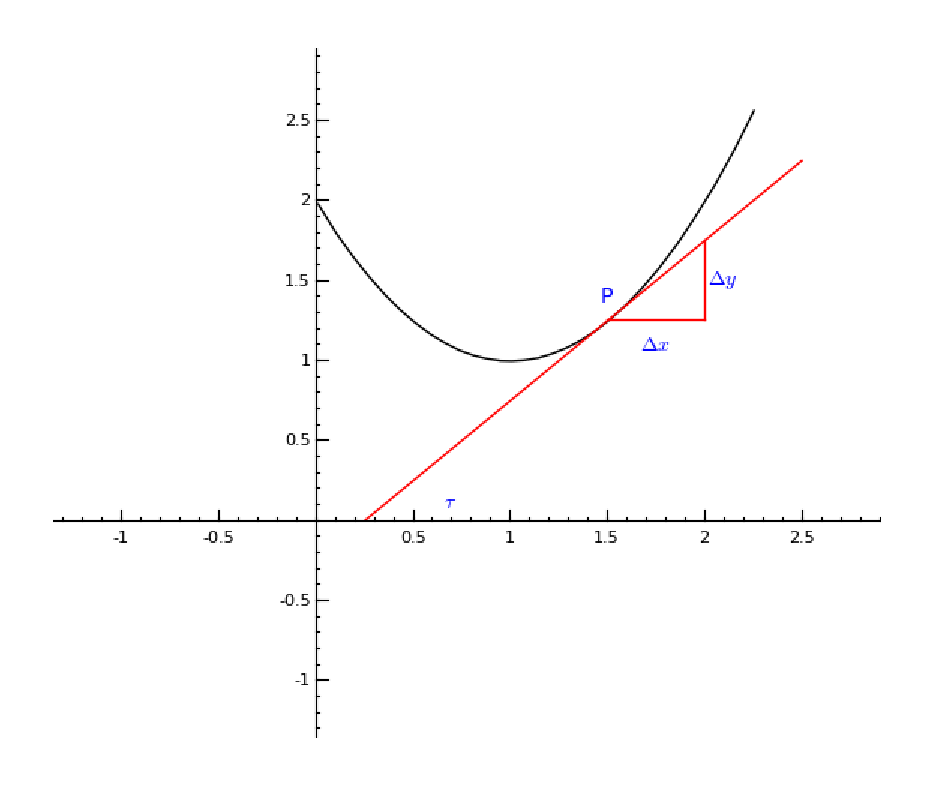
\includegraphics[height=6cm,width=9cm]{parabola-tangent3.eps}
\end{center}
\end{minipage}
%\caption{Scan of Granville's graphic of the differential of a function.}
\caption{The differential of a function.}
\label{fig:differential}
\end{figure}
%sage: p1 = plot(1+(x-1)^2, 0,2.25, rgbcolor=(0,0,0))
%sage: p2 = plot(x-1/4, 0.25, 2.5, rgbcolor=(1,0,0))
%sage: p3 = line([[1.5,1.25],[2.0,1.25]], rgbcolor=(1,0,0))
%sage: p4 = line([[2.0,1.25],[2.0,1.75]], rgbcolor=(1,0,0))
%sage: p5 = plot((5/3)*x-1.25, 0.25, 2.5, rgbcolor=(1,0,0))
%sage: t1 = text("P", (1.5,1.4))
%sage: t2 = text("$\\tau$", (0.6, 0.15))
%sage: t3 = text("$\Delta x$", (1.75, 1.1))
%sage: t4 = text("$\Delta y$", (2.1, 1.5))
%sage: t5 = text("Q", (2.1,2.4))
%sage: t6 = text("$\\theta$", (1.0,0.15))
%sage: show(p1+p2+p3+p4+p5+t1+t2+t3+t4+t5+t6)
%%% this is a superset of commands...

Let $f'(x)$ be the derivative of $y = f(x)$ at P. Take $dx = PQ$, then

\[
    dy = f'(x)dx = \tan \tau \cdot PQ = \frac{QT}{PQ} \cdot PQ = QT.
\]
Therefore $dy$, or $df(x)$, is the increment ($= QT$) of 
the ordinate of the tangent corresponding\footnote{The student 
should note especially that the differential ($= dy$) and the 
increment ($= dy$) of the function corresponding to the same 
value of $dx$ ($= Δx$) are not in general equal. For, 
in Figure \ref{fig:differential}, $dy = QT$, but 
$Δy = QP'$.}  to $dx$.

This gives the following interpretation of the derivative as a fraction.

If an arbitrarily chosen increment of the independent 
variable $x$ for a point $(x, y)$ on the curve $y = f(x)$ be 
denoted by $dx$, then in the derivative

\[
    \frac{dy}{dx} = f'(x) = \tan \tau,
\]
$dy$ denotes the corresponding increment of the ordinate 
drawn to the tangent.

%89. 
\section{Infinitesimals}

In the Differential Calculus we are usually concerned 
with the derivative, that is, with the ratio of the 
differentials $dy$ and $dx$. In some applications it is also 
useful to consider $dx$ as an infinitesimal 
(see \S \ref{sec:15}), %§15, p. 13), 
that is, as a variable whose values remain numerically 
small, and which, at some stage of the investigation, approaches 
the limit zero. Then by (\ref{eqn:B-88}), %p. 131, 
and item 2 in \S \ref{sec:20}, %(2), p. 19, 
$dy$ is also an infinitesimal.

In problems where several infinitesimals enter we often 
make use of the following

\begin{theorem}
\label{thrm:89}
%Theorem. 
{\rm 
In problems involving the limit of the ratio of two 
infinitesimals, either infinitesimal may be replaced 
by an infinitesimal so related to it that the limit of 
their ratio is unity.
}
\end{theorem}

\pf
 Let $\alpha$, $\beta$, $\alpha'$, $\beta'$ be 
infinitesimals so related that

\[
%(C) 
\lim \frac{\alpha'}{\alpha} = 1,\ \ \ \lim \frac{\beta'}{\beta} = 1.
\]
We have 

\[
\frac{\alpha}{\beta} 	
= \frac{\alpha'}{\beta'} \cdot \frac{\alpha}{\alpha'} 
\cdot \frac{\beta'}{\beta}
\]
identically, and 

\[
\lim \frac{\alpha}{\beta} 	
= \lim \frac{\alpha '}{\beta '} \cdot \lim \frac{\alpha}{\alpha '} 
\cdot \lim \frac{\beta '}{\beta}
=\lim \frac{\alpha'}{\beta'} \cdot 1 \cdot 1 ,
\]
by Theorem \ref{thrm:II-20}. % 	Th. II, p. 18
Therefore, 

\[
%(D) 	
\lim \frac{\alpha}{\beta} 	= \lim \frac{\alpha'}{\beta'}.
\]
\qed

Now let us apply this theorem to the two following important limits.

For the independent variable $x$, we know from the previous 
section that $\Delta x$ and $dx$ are identical.
Hence their ratio is unity, and also limit 
$\frac{\Delta x}{dx} = 1$. That is, by the above theorem,
%(E) 
In the limit of the ratio of $\Delta x$ and a second infinitesimal, 
$\Delta x$ may be replaced by $dx$.

On the contrary it was shown that, for the dependent variable $y$, 
$\Delta y$ and $dy$ are in general unequal. But we shall now show, however, 
that in this case also
$\lim \frac{\Delta y}{dy} 	= 1$.
Since $\lim_{\Delta x \to 0} \frac{\Delta y}{\Delta x} = f'(x)$ 
we may write $\frac{\Delta y}{\Delta x} 	= f'(x) + \epsilon$,
where $\epsilon$ is an infinitesimal which approaches 
zero when $\Delta x \to 0$.

Clearing of fractions, remembering that $\Delta x \to dx$,
$\Delta y= f'(x)dx + \epsilon \cdot \Delta x$,
or $\Delta y= dy + \epsilon \cdot \Delta x$, 
by (\ref{eqn:B-88}). %, p. 131 [§89]
Dividing both sides by $\Delta y$,
$1 	= \frac{dy}{\Delta y} + \epsilon \cdot \frac{\Delta x}{\Delta y}$,
or $\frac{dy}{\Delta y}	= 1 - \epsilon \cdot \frac{\Delta x}{\Delta y}$.
Therefore, $\lim_{\Delta x \to 0} \frac{dy}{\Delta y} = 1$,
and hence $\lim_{\Delta x \to 0} \frac{\Delta y}{dy} = 1$. 
That is, by the above theorem,
%(F) 
In the limit of the ratio of $\Delta y$ and a second infinitesimal, 
$\Delta y$ may be replaced by $dy$.

%90. 
\section{Derivative of the arc in rectangular coordinates}
\label{sec:90}

Let $s$ be the length\footnote{Defined in integral calculus. 
For now, we simply assume that there is a function $s=s(x)$
such that if you go along the curve from a point $A$ to a point 
$P=(x,y)$ then $s(x)$ describes the length of that arc.}  %§ 209.} 
of the arc AP measured from a fixed point A on the curve.


\begin{figure}[h!]
%\begin{tabular}{cc}
\begin{minipage}{\textwidth}
\begin{center}
%\vspace{1.0 cm}
%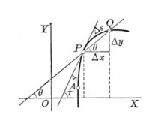
\includegraphics[height=4cm,width=4cm]{derivative-arc.eps}
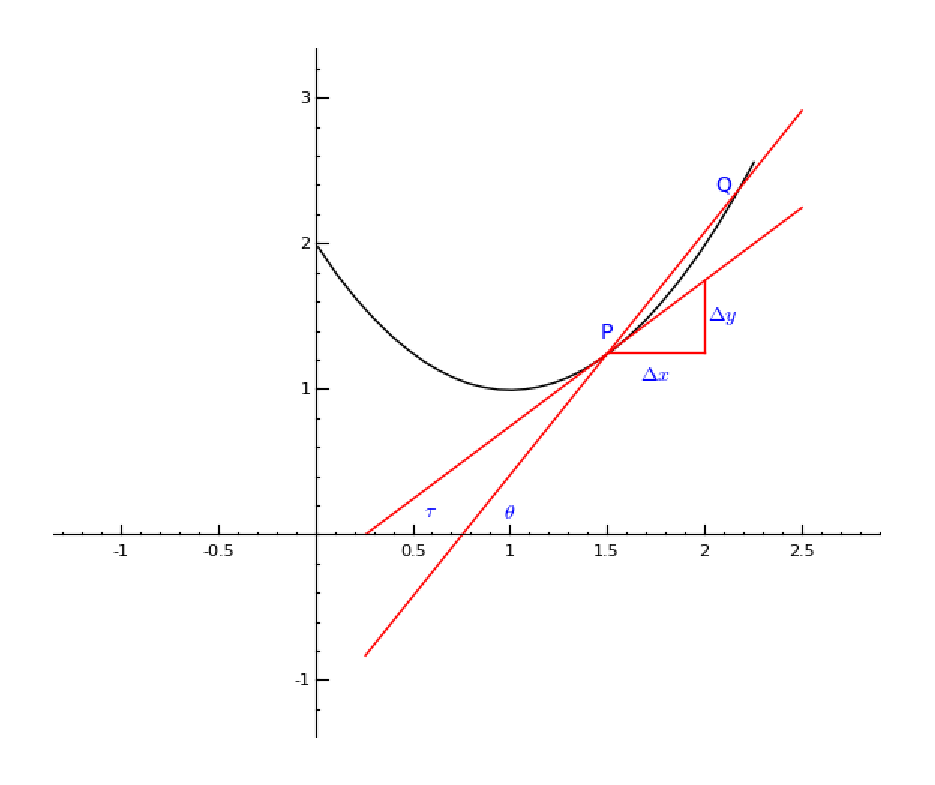
\includegraphics[height=4cm,width=4cm]{parabola-tangent4.eps}
\end{center}
\end{minipage}
%\caption{Scan of Granville's graphic of the differential of the arc length.}
\caption{The differential of the arc length.}
\label{fig:derivative-arc}
\end{figure}
%sage: p1 = plot(1+(x-1)^2, 0,2.25, rgbcolor=(0,0,0))
%sage: p2 = plot(x-1/4, 0.25, 2.5, rgbcolor=(1,0,0))
%sage: p3 = line([[1.5,1.25],[2.17,1.25]], rgbcolor=(1,0,0))
%sage: p4 = line([[2.17,1.25],[2.17,2.38]], rgbcolor=(1,0,0))
%sage: p5 = plot((5/3)*x-1.25, 0.25, 2.5, rgbcolor=(1,0,0))
%sage: t1 = text("P", (1.5,1.4))
%sage: t2 = text("$\\tau$", (0.6, 0.15))
%sage: t3 = text("$\Delta x$", (1.9, 1.1))
%sage: t4 = text("$\Delta y$", (2.3, 1.8))
%sage: t5 = text("Q", (2.1,2.4))
%sage: t6 = text("$\\theta$", (1.0,0.15))
%sage: t7 = text("$\Delta s$", (1.8, 1.9))
%sage: show(p1+p2+p3+p4+p5+t1+t2+t3+t4+t5+t6+t7)


Denote the increment of $s$ (= arc PQ) by $\Delta s$. 
The definition of the length of arc depends on the 
assumption that, as Q approaches P,

\[
    \lim \left ( \frac{\mbox{chord} PQ}{\mbox{arc} PQ} \right ) = 1.
\]
If we now apply Theorem \ref{thrm:89} %on p. 132 [§89] 
to this, we get
%(G) 
In the limit of the ratio of chord PQ and a second infinitesimal, 
chord PQ may be replaced by arc PQ (= $\Delta s$).

From the above figure

\begin{equation}
%(H) 
({\rm chord}\ PQ)^2 = (\Delta x)^2 + (\Delta y)^2,
\label{eqn:H-90}
\end{equation}
Dividing through by $(\Delta x)^2$, we get

\[
%(I)
\left ( \frac{\mbox{chord} PQ}{\Delta x} \right )^2 
= 1 + \left ( \frac{\Delta y}{\Delta x} \right )^2.
\]
Now let Q approach P as a limiting position; then 
$\Delta x \to 0$ and we have

\[
 \left ( \frac{ds}{dx} \right )^2 = 1 + \left ( \frac{dy}{dx} \right )^2.
\]
(Since $\lim_{\Delta x \to 0} \left ( \frac{chord PQ}{\Delta x} \right )
= \lim_{\Delta x \to 0} \left ( \frac{\Delta s}{\Delta x} \right ) 
= \frac{ds}{dx}$.) %, (G).]
Therefore, 

\begin{equation}
%(24)
\frac{ds}{dx} = \sqrt{1 + \left ( \frac{dy}{dx} \right )^2}.
\label{eqn:24-90}
\end{equation}

Similarly, if we divide (\ref{eqn:H-90}) by 
$(\Delta y)^2$ and pass to the limit, we get

\[
%(25) 
\frac{ds}{dy} = \sqrt{\left ( \frac{dx}{dy} \right )^2 + 1}.
\]
Also, from the above figure,

\[
    \cos \theta 
= \frac{\Delta x}{\mbox{chord} PQ},\ \ \  \sin \theta 
= \frac{\Delta y}{\mbox{chord} PQ}.
\]
Now as Q approaches P as a limiting position $\theta \to \tau$, and we get

\begin{equation}
%(26) 
\cos\, \tau = \frac{dx}{ds}, \ \ \ \sin \tau = \frac{dy}{ds}.
\label{eqn:90-26}
\end{equation}
(Since %from (G) 
$\lim \frac{\Delta x}{\mbox{chord} PQ} 
= \lim \frac{\Delta x}{\Delta x} 
= \frac{dx}{ds}$, and 
$\lim \frac{\Delta y}{\mbox{chord} PQ} 
= \lim \frac{\Delta y}{\Delta s} = \frac{dy}{ds}$.)
Using the notation of differentials, these formulas %(24) and (25) 
may be written

\begin{equation}
%(27) 
ds 
= \left [ 1 + \left ( \frac{dy}{dx} \right )^2 \right ]^{\frac{1}{2}} dx
\label{eqn:90-27}
\end{equation}
and

\begin{equation}
%(28) 
ds = \left [ \left ( \frac{dx}{dy} \right )^2 + 1 \right ]^{\frac{1}{2}} dy,
\label{eqn:28-90}
\end{equation}
respectively.
Substituting the value of $ds$ from (\ref{eqn:90-27}) in (\ref{eqn:90-26}),

\begin{equation}
%(29) 
\cos \tau 
= \frac{1}{\left[ 1 + \left ( \frac{dy}{dx} \right )^2 \right]^{\frac{1}{2}}}, 
\ \ \ 
\sin \tau 
= \frac{\frac{dy}{dx}}{\left [ 
1 + \left ( \frac{dy}{dx} \right )^2 \right ]^{\frac{1}{2}}},
\label{eqn:90-29}
\end{equation}
the same relations given by (\ref{eqn:90-26}).

%91. 
\section{Derivative of the arc in polar coordinates}

In the derivation which follows
we shall employ the same figure and the same notation 
used in \S \ref{sec:67}. %on pp, 83, 84. [§67]


\[
({\rm chord}\ PQY)^2 	= (PR)^2 + (RQ)^2
  	= (\rho\sin \Delta \theta)^2 + 
(\rho +  \Delta \rho - \rho\cos \Delta \theta)^2.
\]
Dividing throughout by $(\Delta \theta)^2$, we get

\[
\left( \frac{\mbox{chord} PQ}{\Delta \theta} \right)^2 
= \rho^2 \left( \frac{\sin \Delta \theta}{\Delta \theta} \right)^2 
+ \left( \frac{\Delta \rho}{\Delta \theta} + \rho \cdot 
\frac{1 - \cos \Delta \theta}{\Delta \theta} \right)^2.
\]
Passing to the limit as $\Delta \theta$ diminishes towards zero, 
we get\footnote{Recall: 
$\lim_{\Delta \theta \to 0} \frac{\mbox{chord} PQ}{\Delta \theta} 
= \lim_{\Delta \theta \to 0} \frac{\Delta s}{\Delta \theta} 
= \frac{ds}{d\theta}$, by \S \ref{sec:90};% 	By (G), p. 134 [§90]
$\lim_{\Delta \to 0} \frac{\sin \Delta \theta}{\Delta \theta} = 1$,
by \S \ref{sec:22}; %. 	By §22, p. 21
$\lim_{\Delta \theta \to 0} 
\frac{1 - \cos \Delta \theta}{\Delta \theta} 
= \lim_{\Delta \theta \to 0} 
\frac{2 \sin^2 \frac{\Delta \theta}{2}}{\Delta \theta} 
= \lim_{\Delta \theta \to 0} 
\sin \frac{\Delta \theta}{2} \cdot 
\frac{\sin \frac{\Delta \theta}{2}}{\frac{\Delta \theta}{2}} 
= 0 \cdot 1 = 0$, by \S \ref{sec:22} and 39 in \S \ref{sec:1}.
% 	By 39, p. 2 [§1], and §22, p. 21.
}

\[
\left( \frac{ds}{d\theta} \right)^2 	
= \rho^2 + \left ( \frac{d\rho}{d\theta} \right )^2,
\]
\begin{equation}
%(30) 	
\frac{ds}{d\theta}= \sqrt{\rho^2 + 
\left ( \frac{d\rho}{d\theta} \right )^2}.
\label{eqn:30-91}
\end{equation}
In the notation of differentials this becomes

\begin{equation}
%(31) 	
\ ds =	
\left[ \rho^2 + 
\left( \frac{d\rho}{d\theta} \right)^2 \right]^{\frac{1}{2}} d\theta.
\label{eqn:31-91}
\end{equation}
These relations between $\rho$ and the differentials 
$ds$, $d\rho$, and $d\theta$ are correctly represented by 
a right triangle whose hypotenuse is $ds$ and whose sides are 
$d\rho$ and $\rho d\theta$. Then

\[
    ds = \sqrt{(\rho d\theta)^2 + (d\rho)^2},
\]
and dividing by $ d\theta$ gives (\ref{eqn:30-91}).
Denoting by $\psi$ the angle between $d\rho$ and 
$ds$, we get at once

\[
    \tan \psi = \rho \frac{d\theta}{d\rho},
\]
which is the same as ((\ref{eqn:A-67}). %, p. 84.

\begin{example}
{\rm
Find the differential of the arc of the circle $x^2 + y^2 = r^2$.

Solution. Differentiating, $\frac{dy}{dx} = -\frac{x}{y}$.

To find $ds$ in terms of $x$ we substitute in (\ref{eqn:90-27}), giving

\[
    ds 
= \left[ 1 + \frac{x^2}{y^2} \right]^{\frac{1}{2}} dx 
= \left[ \frac{y^2 + x^2}{y^2} \right]^{\frac{1}{2}} dx 
= \left[ \frac{r^2}{y^2} \right]^{\frac{1}{2}} dx 
= \frac{r dy}{\sqrt{r^2 - x^2}}.
\]
To find $ds$ in terms of $y$ we substitute in (\ref{eqn:28-90}), giving

\[
    ds 
= \left[ 1 + \frac{y^2}{x^2} \right]^{\frac{1}{2}} dy 
= \left[ \frac{x^2 + y^2}{x^2} \right]^{\frac{1}{2}} dy 
= \left[ \frac{r^2}{x^2} \right]^{\frac{1}{2}} 
= \frac{r dy}{\sqrt{r^2 - y^2}}. 
\]
}
\end{example}


\begin{example}
{\rm
Find the differential of the arc of the cardioid 
$\rho = a(l -\cos\theta)$ in terms of $\theta$.

Solution. Differentiating, $\frac{d\rho}{d\theta} = a \sin \theta$.

Substituting in (\ref{eqn:31-91}), gives

\[
ds 
= [ a^2(1 - \cos \theta)^2+ a^2 \sin^2 \theta ]^{\frac{1}{2}} d\theta 
= a [2 - 2\cos \theta]^{\frac{1}{2}} d\theta 
= a \left [ 4 \sin^2 \frac{\theta}{2} \right ]^{\frac{1}{2}} d\theta 
= 2a \sin \frac{\theta}{2} d\theta.
\]
}
\end{example}

\section{Exercises}

Find the differential of arc in each of the following curves:

\begin{enumerate}

\item
%1
$y^2 = 4x$. 	

Ans. 	$ds = \sqrt{\frac{1 + x}{x}}dx$.

\item
%2
$y = ax^2$. 

Ans. $ds = \sqrt{1 + 4a^2 x^2}dx$.

\item
%3
$y = x^3$. 

Ans. $ds = \sqrt{1 + 9x^4}dx$.

\item
%4
$y^3 = x^2$.

Ans. $ds = \frac{1}{2}\sqrt{4 + 9y}dy$.

\item
%5
$x^{\frac{2}{3}} + y^{\frac{2}{3}} = a^{\frac{2}{3}}$.

Ans. $ds = \sqrt[3]{\frac{a}{y}} dy$.

\item
%6
$b^2x^2 + a^2y^2 = a^2b^2$. 

Ans. $ds = \sqrt{\frac{a^2 - e^2 x^2}{a^2 - x^2}} dx$.

\item
%7
$e^y\cos\, x = 1$.

Ans. $ds = \sec\ x\ dx$.

\item
%8
$\rho  = a\cos\theta$.

Ans. $ds = a\ d\theta$.

\item
%9
$\rho^2 = a^2\cos\, 2\theta$. 

Ans. $ds = \sqrt{\sec 2\theta} d\theta$.

\item
%10
$\rho = ae^{\theta \cot\, a}$. 	

Ans. $ds = \rho\csc\, a\cdot d\theta$.

\item
%11
$\rho = a\theta$. 

Ans. $ds = a^{\theta} \sqrt{1 + \log^2 a} d\theta$.

\item
%12
$\rho = a\theta$. 	

Ans. $ds = \frac{1}{a} \sqrt{a^2 + \rho^2} d\rho$.

\item
%13

\[
\begin{array}{ll}
(a)\ \  x^2 - y^2 = a^2. &	(h)\ \  x^{\frac{1}{2}} + y^{\frac{1}{2}} = a^{\frac{1}{2}}.\\
(b)\ \  x^2 = 4ay. &	(i)\ \  y^2 = ax^3.\\
(c)\ \  y = e^x + e^{- x}.  &	(j)\ \  y = \log\, x.\\
(d)\ \  xy = a.  &	(k)\ \  4x = y^3.\\
(e)\ \  y = \log\sec\,x.  &	(l)\ \  \rho = a \sec^2 \frac{\theta}{2}.\\
(f)\ \  \rho  = 2a\tan\theta \sin\theta .  &	(m)\ \  \rho  = 1 + \sin\theta .\\
(g)\ \  \rho = a \sec^3 \frac{\theta}{3}.  &	(n)\ \  \rho \theta  = a.\\
\end{array}
\]

\end{enumerate}


%92. 
\section{Formulas for finding the differentials of functions}

Since the differential of a function is its derivative multiplied 
by the differential of the independent variable, it follows at 
once that the formulas for finding differentials are the same 
as those for finding derivatives given in \S \ref{sec:33}, %§ 33, pp. 34-36, 
if we multiply each one by $dx$.

This gives us

\begin{itemize}
\item[I]
$  	d(c) 	= 0.$

\item[II] 
$	  	d(x) 	= dx.$
\item[III] 
$	  	d(u + v - w) 	= du + dv - dw.$
\item[IV] 
$	  	d(cv) 	= cdv.$
\item[V] 	
$  	d(uv) 	= udv + vdu$.
\item[VI] 
$	  	d(v^n) 	= nv^{n - 1}dv$.
\item[VIa] 
$	d(x^n) 	= nx^{n-1}dx$.
\item[VII] 	
$  	d \left ( \frac{u}{v} \right ) 	= \frac{v du - u dv}{v^2}$.
\item[VIIa] 
$	d \left ( \frac{u}{c} \right ) 	= \frac{du}{c}$.
\item[VIII] 
$	  	d(\log\, av) 	= \log_a e \frac{dv}{v}$.
\item[IX] 	 $ 	d(a^v) 	= a^v\log\, a dv$.
\item[IXa] $	d(e^v) = 	e^vdv$.
\item[X] 	
$  	d(u^v) 	= vu^{v-1} du + \log u \cdot u^v \cdot dv$.
\item[XI] 
$ 	d(\sin\, v) 	= \cos\, v dv$.
\item[XII] 	
$  	d(\cos\, v) 	= -\sin\, vdv$.
\item[XIII] 
$	  	d(\tan\,v) 	= \sec^2vdv$, etc.
\item[XVIII] 	  
$	d(\arcsin\,v) 	= \frac{dv}{\sqrt{1 - v^2}}$, etc.
\end{itemize}

The term ``differentiation'' also includes the operation of finding differentials.

In finding differentials the easiest way is to find the derivative 
as usual, and then multiply the result by $dx$.


\begin{example}
{\rm
Find the differential of

\[
 	\ y 	= \frac{x + 3}{x^2 + 3}.
\]
Solution. 
$dy = d \left( \frac{x + 3}{x^2 + 3} \right) 	
= \frac{(x^2 + 3)d(x + 3) - (x + 3)d(x^2 + 3)}{(x^2 + 3)^2}
= \frac{(x^2 + 3)dx - (x + 3) 2x dx}{(x^2 + 3)^2} 	
= \frac{(3 - 6x - x^2)dx}{(x^2 + 3)^2}.
$
}
\end{example}

\begin{example}
{\rm
Find $dy$ from $b^2x^2 - a^2y^2=a^2b^2$.

Solution. $2b^2xdx - 2a^2ydy =	0$. Therefore, $dy= \frac{b^2 x}{a^2 y} dx$. 
}
\end{example}

\begin{example}
{\rm
Find $dy$ from $\rho^2 	= a^2\cos2\theta$.

Solution. $2\rho d\rho
= -a^2 \sin 2\theta \cdot 2d\theta$.
Therefore, $d\rho= -\frac{a^2 \sin 2\theta}{\rho} d\theta$.
}
\end{example}

\begin{example}
{\rm
Find $d[\arcsin(3t - 4t^3)]$.

Solution. $d[ \arcsin (3t - 4t^3) ] 
= \frac{d(3t - 4t^3)}{\sqrt{1 - (3t - 4t^3)^2}} 
= \frac{3 dt}{\sqrt{1 - t^2}}$.
}
\end{example}


%93. 
\section{Successive differentials}

As the differential of a function is in general also a function of the 
independent variable, we may deal with its differential.
Consider the function

\[
    y = f(x).
\]
$d(dy)$ is called the {\it second differential} of $y$ 
(or of the function) and is denoted by the symbol
\index{second differential}

\[
   d^2y.
\]
Similarly, the third differential of $y$, $d[d(dy)]$, is written
$d^3y$, and so on, to the {\it $n$-th differential of $y$},

\[
   d^ny. 
\]

Since $dx$, the differential of the independent variable, is 
independent of $x$ (see \S \ref{sec:88}), % p. 131 [§88]), 
it must be treated as a constant when differentiating with 
respect to $x$. Bearing this in mind, we get very simple 
relations between successive differentials and successive derivatives.

For 	$dy 	= f'(x)dx$,
and 	$d^2y 	= f''(x)(dx)^2$,
since $dx$ is regarded as a constant.
Also, 	$d^3y 	= f'''(x)(dx)^3$,
and in general 	$d^ny 	= f^{(n)}(x)(dx)^n$.

Dividing both sides of each expression by the power of $dx$ occurring on 
the right, we get our ordinary derivative notation

\[
    \frac{d^2 y}{dx^2} = f''(x), 
\frac{d^3 y}{dx^3} = f'''(x), \dots, 
\frac{d^n y}{dx^n} = f^{(n)} (x).
\]
Powers of an infinitesimal are called {\it infinitesimals of a higher order}. 
\index{infinitesimals}
More generally, if for the infinitesimals $a$ and $b$, then $b$ is said 
to be an infinitesimal of a higher order than $a$.

\begin{example}
{\rm
Find the third differential of
$y =	x^5 - 2x^3 + 3x - 5$.

Solution. $dy 	= (5x^4 - 6x^2 + 3)dx$,
  	$d^2y 	= (20x^3 - 12x)(dx)^2$,
  	$d^3y 	= (60x^2 - 12)(dx)^3$. .

NOTE. This is evidently the third derivative of the function 
multiplied by the cube of the differential of the independent 
variable. Dividing through by $(dx)^3$, we get the third derivative

\[
    \frac{d^3 y}{dx^3} = 60x^2 - 12. 
\]
}
\end{example}

\section{Examples}

Differentiate the following, using differentials:


\begin{enumerate}

\item
%1
$y = ax^3 - bx^2 + cx + d$. 	

Ans. 	$dy = (3ax^2 - 2bx + c)dx$.

\item
%2
$y = 2x^{\frac{5}{2}} - 3x^{\frac{2}{3}} + 6x^{-1} + 5$. 

Ans. $dy = (5x^{\frac{3}{2}} - 2x^{-\frac{1}{3}} - 6x^{-2})dx$.

\item
%3
$y = (a^2 - x^2)^5$. 

Ans. $dy = - 10x(a^2 - x^2)^4dx$.

\item
%4
$y = \sqrt{1 + x^2}$.

Ans. $dy = \frac{x}{\sqrt{1 + x^2}} dx$.

\item
%5
$y = \frac{x^{2n}}{(1 + x^2)^n}$. 

Ans. $dy = \frac{2nx^{2n - 1}}{(1 + x^2)^{n + 1}} dx$.

\item
%6
$y = \log \sqrt{1 - x^3}$.

Ans. $dy = \frac{3x^2 dx}{2(x^3 - 1)}$.

\item
%7
$y = (e^x + e^{-x})^2$. 

Ans. $dy = 2(e^{2x} - e^{-2x})dx$.

\item
%8
$y = e^x\log\, x$. 	

Ans. $dy = e^x \left ( \log x + \frac{1}{x} \right ) dx$.

\item
%9
$s = t - \frac{e^t - e^{-t}}{e^t + e^{-t}}$. 

Ans. $ds = \left ( \frac{e^t - e^{-t}}{e^t + e^{-t}} \right )^2 dt$.

\item
%10
$\rho = \tan\psi + \sec\psi$.

Ans. $ 	d\rho = \frac{1 + \sin \psi}{\cos^2 \psi} d\psi$.

\item
%11
$r = \frac{1}{3} \tan^3 \theta \tan \theta$. 

Ans. $dr = \sec^4\theta d\theta$.

\item
%12
$f(x) = (\log\, x)^3$. 	  	

Ans. $f'(x) dx = \frac{3(\log x)^2 dx}{x}$.
\item
%13
$\psi(t) = \frac{t^3}{(1 - t^2)^{\frac{3}{2}}}$. 	  

Ans. $\psi'(t) dt = \frac{3 t^2 dt}{(1 - t^2)^{\frac{5}{2}}}$.

\item
%14
$d \left [ \frac{x \log x}{1 - x} + \log(1 - x) \right ] = \frac{\log x dx}{(1 - x)^2}$.

\item
%15
$d [ \arctan \log y] = \frac{dy}{y[1 + (\log y)^2]}$.

\item
%16
$d \left [ r \operatorname{arcvers} \frac{y}{r} - \sqrt{2ry - y^2} \right ] 
= \frac{y dy}{\sqrt{2ry - y^2}}$.

\item
%17
$d \left [ \frac{\cos \psi}{2 \sin^2 \psi} - \frac{1}{2} \log \tan \frac{\psi}{2} \right ] 
= -\frac{d\psi}{\sin^3 \psi}$.

\end{enumerate}
